
\documentclass[11pt,compress,t,notes=noshow]{beamer}

\usepackage[english]{babel}
\usepackage{dsfont}
\newcommand\bmmax{2}
\usepackage{bm}
\usepackage{bbm}
\usepackage{verbatim}
\usepackage{amsmath}
\usepackage{amsfonts}
\usepackage{csquotes}
\usepackage{multirow}
\usepackage{longtable}
\usepackage{enumerate}
\usepackage[absolute,overlay]{textpos}
\usepackage{psfrag}
\usepackage{algorithm}
\usepackage{algorithmicx}
\usepackage{algpseudocode}
\usepackage{eqnarray}
\usepackage{multimedia}
\usepackage{media9}
\usepackage{arydshln}
\usepackage{tabularx}
\usepackage{placeins}
\usepackage{tikz}
\usepackage{setspace}
\usepackage{wrapfig}
\usepackage{tcolorbox}
\usepackage[export]{adjustbox}
\usepackage{siunitx}
\usetikzlibrary{shapes,arrows,automata,positioning,calc}
\tikzset{
  %Define standard arrow tip
  >=stealth',
  %Define style for boxes
  punkt/.style={
    rectangle,
    rounded corners,
    draw=black, very thick,
    text width=6.5em,
    minimum height=2em,
    text centered},
  % Define arrow style
  pil/.style={
    ->,
    thick,
    shorten <=2pt,
    shorten >=2pt,}
}
\usepackage{subfig}

%new environments

\newenvironment{vbframe}  %frame with breaks and verbatim
{
 \begin{frame}[containsverbatim,allowframebreaks]
}
{
\end{frame}
}

\newenvironment{vframe}  %frame with verbatim without breaks (to avoid numbering one slided frames)
{
 \begin{frame}[containsverbatim]
}
{
\end{frame}
}

\newenvironment{blocki}[1]   % itemize block
{
 \begin{block}{#1}\begin{itemize}
}
{
\end{itemize}\end{block}
}

\newenvironment{fragileframe}[2]{  %fragile frame with framebreaks
\begin{frame}[allowframebreaks, fragile, environment = fragileframe]
\frametitle{#1}
#2}
{\end{frame}}


\newcommand{\myframe}[2]{  %short for frame with framebreaks
\begin{frame}[allowframebreaks]
\frametitle{#1}
#2
\end{frame}}

\newcommand{\remark}[1]{
  \textbf{Remark:} #1
}

%%%%%%%%%%%%%%%%%%%%%%%%%%%%%%%%%%%%%%%%%%%%%%%%%%%%%%%%%%%%%%%%%%%%%%%%%%%%%%%

% basic latex stuff
\newcommand{\pkg}[1]{{\fontseries{b}\selectfont #1}} %fontstyle for R packages
\newcommand{\lz}{\vspace{0.5cm}} %vertical space
\newcommand{\dlz}{\vspace{1cm}} %double vertical space
\newcommand{\oneliner}[1] % Oneliner for important statements
{\begin{block}{}\begin{center}\begin{Large}#1\end{Large}\end{center}\end{block}}


%\usetheme{lmu-lecture}
\usepackage{../style/lmu-lecture}

\let\code=\texttt
\let\proglang=\textsf

\setkeys{Gin}{width=0.9\textwidth}



\title{Deep Learning}
\author{David Rügamer}
\institute{Department of Statistics -- LMU Munich}
\date{Winter Semester 2021}

\setbeamertemplate{frametitle}{\expandafter\uppercase\expandafter\insertframetitle}

%\begin{document}
%\sloppy
%\end{document}


\input{../../latex-math/basic-math}
\input{../../latex-math/basic-ml}
\input{../../latex-math/ml-nn}

\newcommand{\Dsubtrain}{\mathcal{D}_{\text{subtrain}}}
\newcommand{\Dval}{\mathcal{D}_{\text{val}}}

\begin{document}

\lecturechapter{3}{Early Stopping}
\lecture{Deeplearning}

%%%%%%%%%%%%%%%%%%%%%%%%%%%%%%%%%%%%%%%%%%%%%%%%%%%%%%%%%%%%%%%%%%

\begin{vbframe}{Early Stopping}
  
  \begin{itemize}
    \item When training with an iterative optimizer such as SGD, it is commonly the case that after a certain number of iterations, generalization error begins to increase even though training error continues to decrease.     
    \item \textbf{Early stopping} refers to stopping the algorithm early, before the generalization error increases.
  \end{itemize}
  \begin{figure}
    \centering
      \scalebox{0.5}{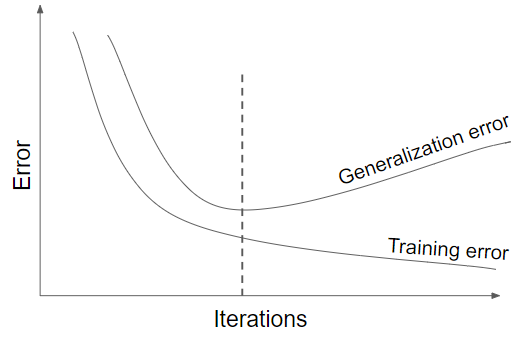
\includegraphics{plots/earlystop.png}}
      \caption{After a certain number of iterations, the algorithm begins to overfit.}
  \end{figure}
\framebreak
   \begin{algorithm}[H]
  \footnotesize
  \caption{Early Stopping}
    \begin{algorithmic}[1]
      \State Initalize $\thetab$ and set $\nu^* = \infty$
      \State Split training data $\Dtrain$ into $\mathcal{D}_{\text{subtrain}}$ and $\mathcal{D}_{\text{val}}$ (e.g. with a ratio of 2:1)
      \While{stop criterion not met: }
        \State Update $\thetab$ using $\mathcal{D}_{\text{subtrain}}$ for a predefined number of optimization steps
        \State Evaluate the model on $\mathcal{D}_{\text{val}}$ and save the resulting validation set error in $\nu$
        \If{$\nu < \nu^*$: }
          \State $ \boldsymbol{\theta}^* \leftarrow \thetab$
          \State $\nu^* \leftarrow \nu$
        \EndIf
      \EndWhile
      \State \,  Return $\boldsymbol{\theta}^*$ 
    \end{algorithmic}
  \end{algorithm}
  \begin{itemize}
    \item A possible stopping criterion is the maximum number of times to observe a worsening validation set error after $\boldsymbol{\theta}^*$ was updated.
    \item More sophisticated forms of early stopping also apply cross-validation.
  \end{itemize}
\framebreak
  \begin{table}
    \begin{tabular}{p{4cm}|p{6cm}}
    \textbf{Strengths} & \textbf{Weaknesses} \\
    \hline
    \hline
    Effective and simple & Periodical evaluation of validation error\\
    \hline
    Applicable to almost any model without adjustment \note{of objective function, parameter space, training procedure} & Temporary copy of $\thetab$ (we have to save $\thetab$ as $\boldsymbol{\theta}^*$ each time the validation error improves) \\
    \hline
    Combinable with other regularization methods & Less data for training $\rightarrow$ include $\mathcal{D}_{\text{val}}$ afterwards
    \end{tabular}
  \end{table}
  \framebreak
  \begin{itemize}
    \item Early stopping restricts the parameter space: Assuming the gradient is bounded, restricting both the number of iterations and the learning rate limits the volume of parameter space reachable from initial parameters.
      \item For a simple linear model and quadratic error function the following relation between optimal early stopping iteration $T_{\text{stop}}$ and weight decay penalization parameter $\lambda$ for learning rate $\alpha$ holds (see Goodfellow et al. (2016) ch. 7.8 for proof):
  \end{itemize}
    \begin{equation*}
      T_{\text{stop}} \approx \frac{1}{\alpha \lambda} 
        \Leftrightarrow \lambda \approx \frac{1}{T_{\text{stop}} \alpha}
    \end{equation*}
  \begin{itemize}
    \item Small $\lambda$ (low penalization) $\Rightarrow$ high $T_{\text{stop}}$ (complex model/lots of updates).
  \end{itemize}
\framebreak
  \begin{figure}
    \centering
      \scalebox{0.85}{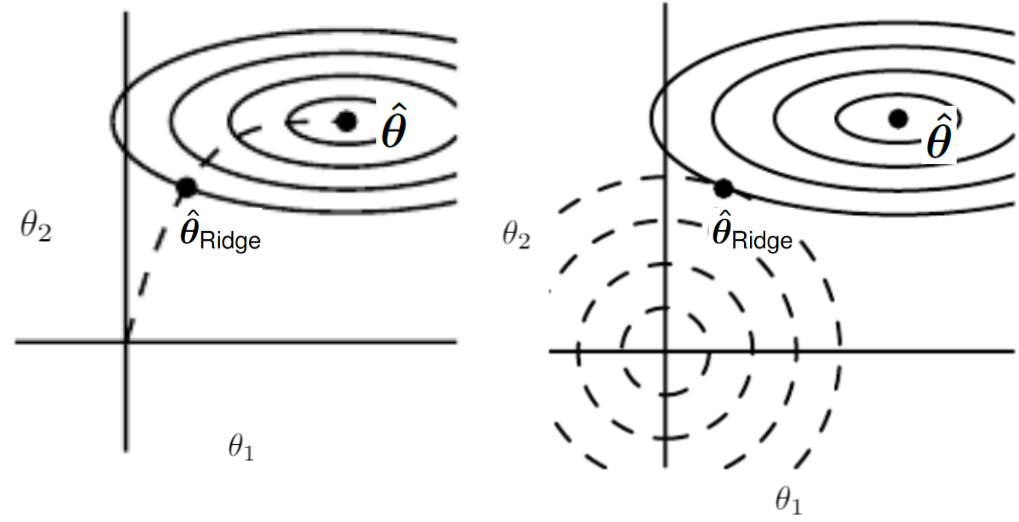
\includegraphics{plots/earlystop_int_hat.png}}
      \tiny{\\ Credit: Goodfellow et al. (2016), ch. 7}
      \caption{\footnotesize An illustration of the effect of early stopping. \textit{Left:} The solid contour lines indicate the contours of the negative log-likelihood. The dashed line indicates the trajectory taken by SGD beginning from the origin. Rather than stopping at the point $\thetah$ that minimizes the risk, early stopping results in the trajectory stopping at an earlier point $\hat{\thetab}_{\text{Ridge}}$. \textit{Right:} An illustration of the effect of L2 regularization for comparison. The dashed circles indicate the contours of the L2 penalty, which causes the minimum of the total cost to lie nearer the origin than the minimum of the unregularized cost.}
  \end{figure}
\end{vbframe}
%%%%%%%%%%%%%%%%%%%%%%%%%%%%%%%%%%%%%%%%%%%%%%%%%%%
%%%%%%%%%%%%%%%%%%%%%%%%%%%%%%%%%%%%%%%%%%%%%%%%%%%%%%%%%%%%%%%%%%
%\section{References}
%%%%%%%%%%%%%%%%%%%%%%%%%%%%%%%%%%%%%%%%%%%%%%%%%%%%%%%%%%%%%%%%%%
%%%%%%%%%%%%%%%%%%          REFERENCES          %%%%%%%%%%%%%%%%%%
%%%%%%%%%%%%%%%%%%%%%%%%%%%%%%%%%%%%%%%%%%%%%%%%%%%%%%%%%%%%%%%%%%
\begin{vbframe}
\frametitle{References}
\footnotesize{
\begin{thebibliography}{99}
%%%%%%%%%%%%%%%%%%%%%%%%%%%%%%%%%%
\bibitem[Ian Goodfellow et al., 2016]{1} Ian Goodfellow, Yoshua Bengio and Aaron Courville (2016)
\newblock Deep Learning
\newblock \emph{\url{http://www.deeplearningbook.org/}}
%%%%%%%%%%%%%%%%%%%%%%%%%%%%%%%%%%
\bibitem[Hastie et al., 2009]{2} Trevor Hastie, Robert Tibshirani and Jerome Friedman (2009)
\newblock The Elements of Statistical Learning
\newblock \emph{\url{https://statweb.stanford.edu/\%7Etibs/ElemStatLearn/}}
\end{thebibliography}
}
\end{vbframe}

\endlecture
\end{document}
